% !TEX program = xelatex
\ifdefined\MASTERBOOK\else
\documentclass[UTF8,zihao=-4,oneside,openany]{ctexbook}

\usepackage[a4paper,top=20mm,bottom=22mm,left=19mm,right=19mm,headheight=24pt]{geometry}
\usepackage[table]{xcolor}
\usepackage{amsmath,amssymb,mathtools,bm}
\usepackage{siunitx}
\usepackage{booktabs,tabularx,array,multicol}
\usepackage{enumitem}
\usepackage{tikz}
\usetikzlibrary{arrows.meta,positioning,calc,angles,quotes}
\usepackage[most]{tcolorbox}
\usepackage{fancyhdr}
\usepackage{hyperref}

% ---------- Theme ----------
\definecolor{Ink}{HTML}{202326}
\definecolor{DeepBlue}{HTML}{294E69}
\definecolor{Blue}{HTML}{47687D}
\definecolor{PaleBlue}{HTML}{F3F5F6}
\definecolor{Gold}{HTML}{6E777D}
\definecolor{PaleGold}{HTML}{F6F6F5}
\definecolor{Green}{HTML}{5B6D76}
\definecolor{PaleGreen}{HTML}{F3F5F6}
\definecolor{Alert}{HTML}{666B6F}
\definecolor{PaleAlert}{HTML}{F6F6F6}
\definecolor{RuleGray}{HTML}{D3D7DA}
\definecolor{TextGray}{HTML}{61686D}

\color{Ink}
\sisetup{
  per-mode=symbol,
  inter-unit-product=\ensuremath{{}\cdot{}},
  exponent-product=\times
}

\hypersetup{
  colorlinks=true,
  linkcolor=DeepBlue,
  urlcolor=Blue,
  pdftitle={高中物理竞赛一轮讲义样章：矢量、坐标系与物理量的分解},
  pdfsubject={高中物理竞赛一轮资料重排样章},
  pdfauthor={物理竞赛一轮资料编写组}
}

\setlength{\parindent}{2em}
\setlength{\parskip}{0.25em}
\setlist{nosep,leftmargin=2em}
\setcounter{secnumdepth}{3}
\setcounter{tocdepth}{2}
\numberwithin{equation}{section}
\counterwithin{table}{section}
\allowdisplaybreaks[2]
\emergencystretch=2em

\ctexset{
  chapter={
    format=\raggedright\LARGE\bfseries\color{Ink},
    titleformat=\LARGE\bfseries\color{Ink},
    beforeskip=0pt,
    afterskip=18pt
  },
  section={
    format=\Large\bfseries\color{DeepBlue},
    beforeskip=1.8ex,
    afterskip=1.0ex
  },
  subsection={
    format=\large\bfseries\color{Ink},
    beforeskip=1.5ex,
    afterskip=0.8ex
  },
  subsubsection={
    format=\normalsize\bfseries\color{Ink}
  }
}

\pagestyle{fancy}
\fancyhf{}
\fancyhead[L]{\small\color{TextGray}高中物理竞赛一轮讲义}
\fancyhead[R]{\small\color{TextGray}第一章\quad 数学与物理工具}
\fancyfoot[C]{\small\color{TextGray}\thepage}
\renewcommand{\headrulewidth}{0.4pt}
\renewcommand{\headrule}{\hbox to\headwidth{\color{RuleGray}\leaders\hrule height \headrulewidth\hfill}}

\newcommand{\vect}[1]{\bm{#1}}
\newcommand{\uvec}[1]{\hat{\vect{#1}}}
\newcommand{\dd}{\mathop{}\!\mathrm{d}}
\DeclareMathOperator{\proj}{proj}

\newtcolorbox{goalbox}{
  enhanced,breakable,
  colback=PaleBlue,colframe=Blue,
  boxrule=0.7pt,arc=2mm,
  title={本节目标},fonttitle=\bfseries,
  coltitle=DeepBlue,
  attach boxed title to top left={xshift=5mm,yshift=-2mm},
  boxed title style={colback=white,colframe=Blue,boxrule=0.7pt,arc=1.5mm}
}

\newtcolorbox[auto counter,number within=section]{examplebox}[2][]{
  enhanced,breakable,
  colback=white,colframe=RuleGray,
  boxrule=0.5pt,arc=0mm,
  title={例题~\thetcbcounter\quad #2},fonttitle=\bfseries,
  coltitle=Ink,colbacktitle=PaleBlue,
  borderline west={1.4pt}{0pt}{DeepBlue},
  #1
}

\newtcolorbox{methodbox}[1]{
  enhanced,breakable,
  colback=PaleGreen,colframe=Green,
  boxrule=0.5pt,arc=0mm,
  title={方法：#1},fonttitle=\bfseries,
  coltitle=Ink,colbacktitle=PaleGreen,
  borderline west={1.2pt}{0pt}{DeepBlue}
}

\newtcolorbox{warningbox}[1]{
  enhanced,breakable,
  colback=PaleAlert,colframe=Alert,
  boxrule=0.5pt,arc=0mm,
  title={易错提醒：#1},fonttitle=\bfseries,
  coltitle=Ink,colbacktitle=PaleAlert,
  borderline west={1.2pt}{0pt}{TextGray}
}

\newtcolorbox{extensionbox}[1]{
  enhanced,breakable,
  colback=PaleGold,colframe=Gold,
  boxrule=0.5pt,arc=0mm,
  title={拓展：#1},fonttitle=\bfseries,
  coltitle=Ink,colbacktitle=PaleGold,
  borderline west={1.2pt}{0pt}{DeepBlue}
}

\newtcolorbox{summarybox}{
  enhanced,breakable,
  colback=PaleBlue,colframe=DeepBlue,
  boxrule=0.9pt,arc=1.5mm,
  title={本节小结},fonttitle=\bfseries,
  coltitle=white,colbacktitle=DeepBlue
}

\newtcolorbox{exercisebox}[1]{
  enhanced,breakable,
  colback=white,colframe=RuleGray,
  boxrule=0.7pt,arc=1.5mm,
  title={#1},fonttitle=\bfseries,
  coltitle=DeepBlue,colbacktitle=PaleBlue
}

\tikzset{
  vector/.style={-{Latex[length=2.5mm]},very thick,draw=DeepBlue},
  component/.style={-{Latex[length=2.2mm]},thick,draw=TextGray},
  axis/.style={-{Latex[length=2mm]},thin,draw=TextGray},
  guide/.style={densely dashed,draw=TextGray}
}

\begin{document}

\pagenumbering{arabic}
\setcounter{page}{1}
\setcounter{chapter}{0}
\chapter{数学与物理工具}
\setcounter{section}{1}
\fi
\ifdefined\MASTERBOOK\clearpage\fi
\section{矢量、坐标系与物理量的分解}

矢量不是“带箭头的数”，而是同时包含大小与方向、并服从特定运算法则的几何对象。
坐标分量只是这个对象在一组基矢下的表示。区分矢量本身与它的分量，是正确处理相对运动、
斜面分解、力矩以及曲线运动的起点。

本节先从正交基下的分解与坐标旋转入手，随后推导点积、投影、叉积和相对速度关系，
重点建立“先写矢量关系、再取有符号分量”的解题习惯。会随位置转动的极坐标基矢需要
乘积法则和链式法则，将在下一节介绍微积分之后完整推导。

{\small\color{TextGray}\noindent\textbf{题源说明：}本节例题为本讲义依据矢量分解、相对运动和
力矩的经典模型自编，未逐字取自特定竞赛原题。\par}

\subsection{标量、矢量与分量}

只有大小而没有空间方向的物理量称为标量，例如质量、时间、温度、能量。既有大小又有方向，并且服从矢量运算法则的物理量称为矢量，例如位移、速度、加速度、力和动量。

“有方向”本身并不足以说明一个量是矢量。例如有限转角在一般情况下不能按平行四边形法则相加。判断的关键是：这个量在坐标系改变时是否按照矢量的变换规律改变。

在一组相互垂直的单位基矢 $\uvec e_x,\uvec e_y,\uvec e_z$ 下，矢量可以表示为
\begin{equation}
  \vect a=a_x\uvec e_x+a_y\uvec e_y+a_z\uvec e_z.
  \label{eq:vector-components}
\end{equation}
正交单位基矢满足
\[
  \uvec e_i\cdot\uvec e_j=\delta_{ij}
  =\begin{cases}
    1,&i=j,\\
    0,&i\ne j.
  \end{cases}
\]
将式 \eqref{eq:vector-components} 分别与三个基矢作点积，可得
\[
  \vect a\cdot\uvec e_x
  =a_x(\uvec e_x\cdot\uvec e_x)
   +a_y(\uvec e_y\cdot\uvec e_x)
   +a_z(\uvec e_z\cdot\uvec e_x)=a_x,
\]
同理
\begin{equation}
  a_x=\vect a\cdot\uvec e_x,\qquad
  a_y=\vect a\cdot\uvec e_y,\qquad
  a_z=\vect a\cdot\uvec e_z.
  \label{eq:components-by-projection}
\end{equation}
所以“求分量”的本质，是把矢量投影到各个单位基矢上。

$\vect a$ 是与坐标系无关的几何对象；$a_x,a_y,a_z$ 是它在当前坐标系中的分量。换一个坐标系，分量会改变，但矢量本身不会改变。由自身点积
\[
  \vect a\cdot\vect a
  =(a_x\uvec e_x+a_y\uvec e_y+a_z\uvec e_z)^2
  =a_x^2+a_y^2+a_z^2
\]
可得其大小
\begin{equation}
  a=\lvert\vect a\rvert=\sqrt{a_x^2+a_y^2+a_z^2}.
  \label{eq:vector-magnitude}
\end{equation}

\begin{center}
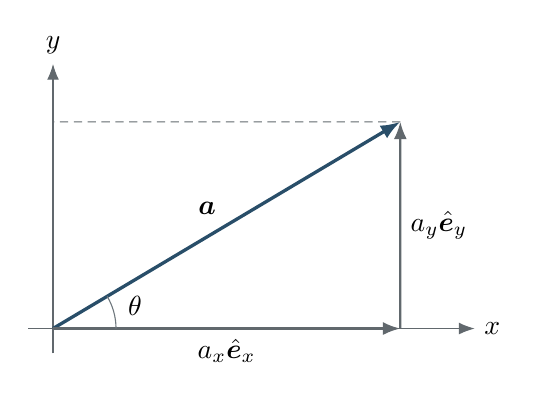
\begin{tikzpicture}[scale=1.05]
  \coordinate (O) at (0,0);
  \coordinate (A) at (4.2,2.5);
  \coordinate (X) at (4.2,0);
  \draw[axis] (-0.3,0)--(5.1,0) node[right] {$x$};
  \draw[axis] (0,-0.3)--(0,3.2) node[above] {$y$};
  \draw[vector] (O)--(A) node[midway,above left] {$\vect a$};
  \draw[component] (O)--(4.2,0) node[midway,below] {$a_x\uvec e_x$};
  \draw[component] (4.2,0)--(A) node[midway,right] {$a_y\uvec e_y$};
  \draw[guide] (A)--(0,2.5);
  \pic[draw=Gold,angle radius=8mm,angle eccentricity=1.35,"$\theta$"] {angle=X--O--A};
\end{tikzpicture}
\end{center}

在二维直角坐标系中，
\[
  a_x=a\cos\theta,\qquad a_y=a\sin\theta.
\]
反过来，可由 $a_x,a_y$ 求得大小和方向。确定方向时应使用分量的正负判断象限，不能只写 $\tan\theta=a_y/a_x$ 后直接取反正切。

\paragraph{坐标轴旋转时分量怎样变化}
设新坐标轴相对原坐标轴逆时针转过 $\varphi$。新基矢在旧基矢下为
\begin{equation}
  \uvec e_{x'}=\cos\varphi\,\uvec e_x+\sin\varphi\,\uvec e_y,
  \qquad
  \uvec e_{y'}=-\sin\varphi\,\uvec e_x+\cos\varphi\,\uvec e_y.
  \label{eq:rotated-basis}
\end{equation}
注意这里转动的是坐标轴，不是矢量。由式 \eqref{eq:components-by-projection}，同一个
$\vect a=a_x\uvec e_x+a_y\uvec e_y$ 在新坐标系中的分量为
\begin{align}
  a_{x'}&=\vect a\cdot\uvec e_{x'}
  =a_x\cos\varphi+a_y\sin\varphi,\label{eq:rotation-x}\\
  a_{y'}&=\vect a\cdot\uvec e_{y'}
  =-a_x\sin\varphi+a_y\cos\varphi.\label{eq:rotation-y}
\end{align}
将两式平方后相加，交叉项相消：
\begin{align*}
  a_{x'}^2+a_{y'}^2
  &=(a_x\cos\varphi+a_y\sin\varphi)^2
    +(-a_x\sin\varphi+a_y\cos\varphi)^2\\
  &=a_x^2(\cos^2\varphi+\sin^2\varphi)
    +a_y^2(\sin^2\varphi+\cos^2\varphi)\\
  &=a_x^2+a_y^2.
\end{align*}
分量随坐标轴转动而改变，矢量的长度却保持不变。这是“矢量本身不依赖坐标系”的
具体代数表现。

\begin{warningbox}{矢量与矢量大小是不同对象}
$\vect v_1=\vect v_2$ 表示大小和方向都相同；$v_1=v_2$ 只表示速率相同。两辆汽车速率相同、行驶方向相反时，它们的速度并不相等。
\end{warningbox}

\subsection{矢量的加减与相对运动}

矢量相加遵循首尾相接或平行四边形法则。若
\[
  \vect a=(a_x,a_y,a_z),\qquad \vect b=(b_x,b_y,b_z),
\]
则
\begin{equation}
  \vect a+\vect b=(a_x+b_x,\ a_y+b_y,\ a_z+b_z).
  \label{eq:vector-add}
\end{equation}
矢量减法就是加上反向矢量：$\vect a-\vect b=\vect a+(-\vect b)$。

\begin{center}
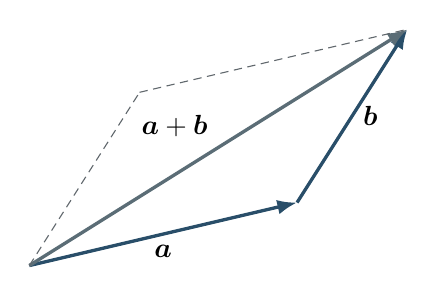
\begin{tikzpicture}[scale=1.0]
  \coordinate (O) at (0,0);
  \coordinate (A) at (3.4,0.8);
  \coordinate (B) at (4.8,3.0);
  \draw[vector] (O)--(A) node[midway,below] {$\vect a$};
  \draw[vector] (A)--(B) node[midway,right] {$\vect b$};
  \draw[vector,draw=Green] (O)--(B) node[midway,above left] {$\vect a+\vect b$};
  \draw[guide] (O)--($(B)-(A)$);
  \draw[guide] ($(B)-(A)$)--(B);
\end{tikzpicture}
\end{center}

相对运动中的速度关系也是矢量加法。以下位置、速度和加速度分量均在同一组彼此平行、
且不随时间转动的基矢中表示；若参考系相对转动，还会出现由基矢变化产生的附加项。
若物体 $A$ 相对 $B$ 的速度为 $\vect v_{A/B}$，$B$ 相对地面的速度为 $\vect v_{B/G}$，则
\begin{equation}
  \vect v_{A/G}=\vect v_{A/B}+\vect v_{B/G}.
  \label{eq:relative-velocity}
\end{equation}
下标必须保持“首尾衔接”：$A/B+B/G=A/G$。

这个关系不是需要额外记忆的规则。以地面 $G$ 为参考，两个物体的位置矢量满足
\begin{equation}
  \vect r_{A/B}=\vect r_{A/G}-\vect r_{B/G}.
  \label{eq:relative-position}
\end{equation}
对时间求导，且各速度均相对于同一时刻定义，得到
\[
  \vect v_{A/B}=\vect v_{A/G}-\vect v_{B/G},
\]
移项即为式 \eqref{eq:relative-velocity}。再次求导还有
\begin{equation}
  \vect a_{A/B}=\vect a_{A/G}-\vect a_{B/G}.
  \label{eq:relative-acceleration}
\end{equation}
当参考物体 $B$ 相对地面做匀速直线运动时，$\vect a_{B/G}=0$，于是两个参考系测得
的加速度相同；若 $B$ 有加速度，就不能再作这样的替换。

\begin{examplebox}{横渡有流速的河}
河宽为 $d$，水流以速度 $v$ 沿河岸向东。小船相对水的速度大小恒为 $u$，且 $u>v$。若要求小船恰好到达正对岸，应朝什么方向行驶？渡河时间是多少？

\tcblower
取东为 $+x$、正对岸为 $+y$。水相对地面的速度为
\[
  \vect v_{\text{水/地}}=v\uvec e_x.
\]
为了使船相对地面的速度没有 $x$ 分量，船相对水的速度必须满足
\[
  v_{\text{船/水},x}=-v.
\]
由 $\lvert\vect v_{\text{船/水}}\rvert=u$ 得
\[
  v_{\text{船/水},y}=\sqrt{u^2-v^2}.
\]
因此船头应偏向上游，且
\[
  \sin\alpha=\frac{v}{u},
  \qquad
  t=\frac{d}{\sqrt{u^2-v^2}},
\]
其中 $\alpha$ 是船头方向与正对岸方向的夹角。
\end{examplebox}

\subsection{点积：投影、功与夹角}

两个矢量的点积定义为
\begin{equation}
  \vect a\cdot\vect b=ab\cos\theta,
  \label{eq:dot-product}
\end{equation}
其中 $\theta$ 是两矢量之间的较小夹角。点积的结果是标量。它把“一个矢量在另一个方向上的有效部分”提取出来。

点积的分量形式可以直接从基矢的正交性推出。把
\[
  \vect a=a_i\uvec e_i,\qquad \vect b=b_j\uvec e_j
\]
代入点积并对重复指标求和：
\begin{align}
  \vect a\cdot\vect b
  &=(a_i\uvec e_i)\cdot(b_j\uvec e_j)
   =a_ib_j(\uvec e_i\cdot\uvec e_j)\notag\\
  &=a_ib_j\delta_{ij}
   =a_xb_x+a_yb_y+a_zb_z.
  \label{eq:dot-product-components}
\end{align}
因此几何定义 $ab\cos\theta$ 与分量计算式并不是两条彼此独立的公式。

设 $\uvec n$ 是某方向的单位矢量，则 $\vect a$ 沿该方向的有符号分量为
\[
  a_n=\vect a\cdot\uvec n.
\]
若要得到平行于 $\vect b$ 的投影矢量，则
\begin{equation}
  \proj_{\vect b}\vect a
  =\frac{\vect a\cdot\vect b}{b^2}\,\vect b.
  \label{eq:vector-projection}
\end{equation}

式 \eqref{eq:vector-projection} 也可以逐步求出。投影矢量与 $\vect b$ 平行，故可设
\[
  \proj_{\vect b}\vect a=\lambda\vect b.
\]
它在 $\vect b$ 方向上的有符号长度应等于 $a\cos\theta$，两边与 $\vect b$ 点积：
\[
  (\lambda\vect b)\cdot\vect b
  =\vect a\cdot\vect b.
\]
于是 $\lambda b^2=\vect a\cdot\vect b$，即
$\lambda=(\vect a\cdot\vect b)/b^2$，代回便得到投影公式。若只求有符号标量分量，
应与单位矢量 $\uvec e_b=\vect b/b$ 点积；若求投影矢量，还要乘回方向。

功正是点积的典型应用。恒力 $\vect F$ 使物体发生位移 $\vect s$ 时，
\[
  W=\vect F\cdot\vect s=Fs\cos\theta.
\]
只有沿位移方向的力分量做功。

\begin{examplebox}{斜面上的重力分解}
质量为 $m$ 的物体位于倾角为 $\alpha$ 的斜面上。取 $\uvec e_t$ 沿斜面向上，$\uvec e_n$ 垂直斜面向外，写出重力的两个分量。

\tcblower
\begin{center}
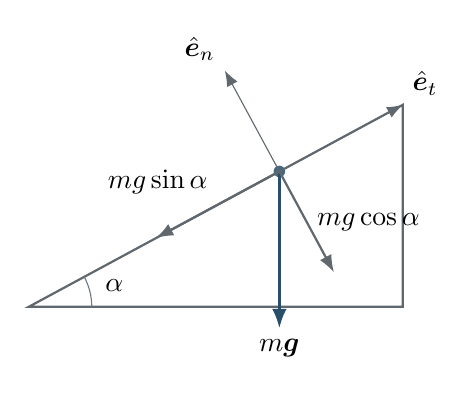
\begin{tikzpicture}[scale=0.95]
  \coordinate (A) at (0,0);
  \coordinate (B) at (5,0);
  \coordinate (C) at (5,2.7);
  \coordinate (P) at (3.35,1.81);
  \draw[thick,draw=TextGray] (A)--(B)--(C)--cycle;
  \fill[Blue] (P) circle (2.2pt);
  \draw[vector] (P)--++(0,-2.1) node[below] {$m\vect g$};
  \draw[component] (P)--++(-1.65,-0.89) node[midway,above left] {$mg\sin\alpha$};
  \draw[component] (P)--++(0.73,-1.35) node[midway,right] {$mg\cos\alpha$};
  \draw[axis] (P)--++(1.65,0.89) node[above right] {$\uvec e_t$};
  \draw[axis] (P)--++(-0.73,1.35) node[above left] {$\uvec e_n$};
  \pic[draw=Gold,angle radius=8mm,angle eccentricity=1.4,"$\alpha$"] {angle=B--A--C};
\end{tikzpicture}
\end{center}
由投影关系，
在水平向右、竖直向上的直角坐标中，重力为
\[
  \vect F_g=(0,-mg).
\]
沿斜面向上和垂直斜面向外的单位基矢分别为
\[
  \uvec e_t=(\cos\alpha,\sin\alpha),
  \qquad
  \uvec e_n=(-\sin\alpha,\cos\alpha).
\]
用点积求有符号分量：
\begin{align*}
  F_t&=\vect F_g\cdot\uvec e_t
  =(0,-mg)\cdot(\cos\alpha,\sin\alpha)
  =-mg\sin\alpha,\\
  F_n&=\vect F_g\cdot\uvec e_n
  =(0,-mg)\cdot(-\sin\alpha,\cos\alpha)
  =-mg\cos\alpha.
\end{align*}
因此
\[
  m\vect g=-mg\sin\alpha\,\uvec e_t-mg\cos\alpha\,\uvec e_n.
\]
分量前的负号说明它们分别沿斜面向下、垂直斜面向内。$mg\sin\alpha$ 和 $mg\cos\alpha$ 是分量大小，不应把负号写进“大小”中。
\end{examplebox}

\begin{methodbox}{先定正方向，再写分量}
分解矢量前先画出单位基矢并明确正方向。之后用点积求有符号分量，而不是只凭图形猜 $\sin$、$\cos$。这样斜面角度变化、坐标轴反向或图形旋转后，方法仍然可靠。
\end{methodbox}

\subsection{叉积：有向面积、力矩与角动量}

两个三维矢量的叉积 $\vect a\times\vect b$ 是一个新矢量，其大小为
\begin{equation}
  \lvert\vect a\times\vect b\rvert=ab\sin\theta,
  \label{eq:cross-product-magnitude}
\end{equation}
方向垂直于 $\vect a,\vect b$ 所在平面，由右手定则确定。叉积具有反交换性：
\[
  \vect a\times\vect b=-\vect b\times\vect a.
\]
在右手直角坐标系中，
\[
  \uvec e_x\times\uvec e_y=\uvec e_z,\qquad
  \uvec e_y\times\uvec e_z=\uvec e_x,\qquad
  \uvec e_z\times\uvec e_x=\uvec e_y.
\]
交换次序，符号取反。

对一般矢量
\[
  \vect a=a_x\uvec e_x+a_y\uvec e_y+a_z\uvec e_z,\qquad
  \vect b=b_x\uvec e_x+b_y\uvec e_y+b_z\uvec e_z,
\]
利用叉积对加法的分配律展开。相同基矢的叉积为零，保留下来的六项按右手定则合并：
\begin{align*}
  \vect a\times\vect b
  ={}&(a_yb_z-a_zb_y)\uvec e_x
   +(a_zb_x-a_xb_z)\uvec e_y\\
   &+(a_xb_y-a_yb_x)\uvec e_z.
\end{align*}
这常写成形式行列式
\begin{equation}
  \vect a\times\vect b=
  \begin{vmatrix}
    \uvec e_x&\uvec e_y&\uvec e_z\\
    a_x&a_y&a_z\\
    b_x&b_y&b_z
  \end{vmatrix}.
  \label{eq:cross-product-components}
\end{equation}
第二个分量展开时带负号，正是最常见的符号错误来源；用循环顺序
$x\to y\to z\to x$ 可以迅速检查。

叉积大小等于由 $\vect a,\vect b$ 张成的平行四边形面积。它在物理中最常见的两个应用是
\begin{equation}
  \vect\tau=\vect r\times\vect F,
  \qquad
  \vect L=\vect r\times\vect p,
  \label{eq:torque-angular-momentum}
\end{equation}
分别表示力矩和角动量。
其中 $\vect r$ 必须从所选参考点指向质点或力的作用点；改变参考点，力矩和角动量一般也会改变。

\begin{examplebox}{力臂为何是垂直距离}
在距转轴位置矢量为 $\vect r$ 的点施加力 $\vect F$，两者夹角为 $\theta$。求力矩大小，并说明什么情况下力矩最大。

\tcblower
由叉积定义，
\[
  \tau=rF\sin\theta=F(r\sin\theta).
\]
$r\sin\theta$ 正是转轴到力的作用线的垂直距离，即力臂。给定 $r$ 和 $F$ 时，$\theta=\ang{90}$，力矩最大；若力的作用线通过转轴，则 $\theta=0$ 或 $\pi$，力矩为零。
\end{examplebox}

\begin{warningbox}{点积和叉积不要混用}
点积得到标量，常用于功、投影和夹角；叉积得到垂直于原平面的矢量，常用于力矩和角动量。$ab\cos\theta$ 与 $ab\sin\theta$ 背后对应的是两种完全不同的几何问题。
\end{warningbox}

\subsection{坐标系不是背景装饰}

建立坐标系需要明确三件事：原点、坐标轴方向和正方向。坐标系本身可以任意选择，但一个好的选择能让约束条件、对称性和运动方向直接表现出来。

\begin{table}[htbp]
\centering
\caption{常见问题的坐标系选择}
\rowcolors{2}{PaleBlue}{white}
\begin{tabularx}{\textwidth}{>{\bfseries}l X X}
\toprule
问题特征 & 推荐坐标 & 主要好处 \\
\midrule
固定斜面 & 一轴沿斜面、一轴垂直斜面 & 支持力只在法向，约束直接 \\
抛体运动 & 水平—竖直直角坐标 & 重力只有一个分量 \\
圆周或有心运动 & 平面极坐标 $(r,\theta)$ & 径向与切向物理意义清楚 \\
碰撞与质心运动 & 一轴沿总动量或碰撞线 & 动量方程分量最少 \\
对称电场、引力场 & 沿对称轴或径向 & 无关分量由对称性直接消失 \\
\bottomrule
\end{tabularx}
\end{table}

\subsection{一套可靠的分解流程}

\begin{methodbox}{建系—画基矢—写矢量—投影—验算}
\begin{enumerate}[label=\arabic*.]
  \item 根据约束和对称性选择原点与坐标轴；
  \item 在图上明确画出正方向单位基矢；
  \item 先写完整矢量方程，再投影到各坐标轴；
  \item 用点积求有符号分量，用叉积处理转动效应；
  \item 检查分量合成后的大小、方向、单位和特殊极限。
\end{enumerate}
\end{methodbox}

\subsection*{分层训练}
\begin{enumerate}[label=\textbf{\arabic*.},leftmargin=2.4em]
  \item \textbf{基础} 已知 $\vect a=(3,4)$、$\vect b=(1,-2)$。求
  $\vect a\cdot\vect b$ 以及 $\vect a$ 在 $\vect b$ 方向上的投影矢量。
  \item \textbf{基础} 河宽为 $d$，水流速度为 $v$，船相对水的速度大小为 $u$。
  若只要求渡河时间最短，船头应指向何方？求最短时间和下游漂移距离。
  \item \textbf{方法} 两质点的相对位置和相对速度分别为 $\vect r_0$、$\vect u$，且
  $\vect u$ 为常矢量。由 $|\vect r_0+\vect u t|^2$ 取极值，求最接近时刻及最小距离。
  说明所得时刻为负时应怎样解释。
  \item \textbf{提升} 力 $\vect F=(F_x,F_y,0)$ 作用于位置
  $\vect r=(x,y,0)$。求关于原点的力矩，并用结果说明“力的作用线通过原点”为什么等价于
  力矩为零。
\end{enumerate}
{\small\color{TextGray}\noindent
参考结果：$\vect a\cdot\vect b=-5$，$\proj_{\vect b}\vect a=(-1,2)$；
$t_{\min}=d/u$、漂移 $vd/u$；若 $\vect r_0\cdot\vect u<0$，
$t_*=-(\vect r_0\cdot\vect u)/u^2$，
$d_{\min}^2=r_0^2-(\vect r_0\cdot\vect u)^2/u^2$；
$\vect\tau=(xF_y-yF_x)\uvec e_z$。\par}

\ifdefined\MASTERBOOK
  \let\sectionfinish\relax
\else
  \def\sectionfinish{\end{document}}
\fi
\sectionfinish
